%BEGIN TICKET 39
\begin{definition}
    $A \subset X$.  $(X, \rho)$ --- метрическая пространство.

     $E \subset A$,  $\eps$-сеть множества  $A$, если  $\forall a \in A \exists x \in E\!: \rho(x, a) < \eps$.

     Конечная  $\eps$-сеть ---  $E$-конечное множество.

     То есть $\{x_1, x_2,.., x_n\} \subset A$ --- $\eps$-сеть, если  $\forall a \in A \exists k\quad \rho(a, x_k) < \eps$.
\end{definition}
\begin{definition}
    $A$ --- вполне ограничено, если  $\forall \eps > 0 \exists$ конечная $\eps$-сеть  $A$.
\end{definition}

\begin{properties}
    \begin{enumerate}
        \item Вполне ограниченность $\implies$ ограниченность.
             \begin{proof}
                $\eps = 1$ и конечная  $1$-сеть  $x_1, x_2,\ldots,x_n$. $A \subset \bigcup\limits_{k=1}^n B_1(x_k) \subset B_{r+1}(x_1)$, где $r = \max\limits_{i \neq j} \rho(x_i, x_j)$.
            \end{proof}
        \item В $\R^d$ ограниченность  $\implies$ вполне ограниченность. 
             \begin{proof}
                $A \subset \R^d$ --- ограниченное.  $A \subset B_R(O) \subset [-R, R]^d$.

                Зафиксируем $\eps > 0$ и возьмем  $n \in \N$.  $\rho(x_i, a) \le$ главная диагональ $=\sqrt{d}\frac{2R}{n} < \eps$ при $n > \frac{\sqrt{d} 2R}{\eps}$ получается $\eps$-сеть ($\sqrt{d}$ --- диагональ в $d$-мерном кубе).
                \begin{figure}[h!]
                    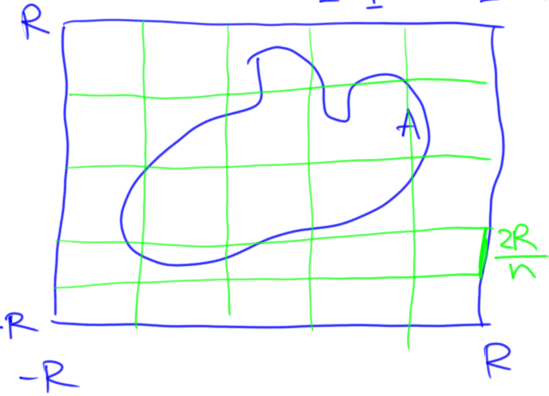
\includegraphics[scale=0.5]{delone_set}
                \end{figure}
            \end{proof}
    \end{enumerate}
\end{properties}
%END TICKET 39